\documentclass{beamer}
\usepackage[utf8]{inputenc}
\usetheme{Copenhagen}
\usecolortheme{default}

\usepackage{graphicx}
\graphicspath{ {../Resources/} }

\title{An Introduction to Git and GitHub}
\author{Lan Peng}
\institute{Department of Industrial and Systems Engineering, University at Buffalo, SUNY}
\date{\today}

\begin{document}
	\frame{\titlepage}
	
	\begin{frame}
		\frametitle{Outline}
		\tableofcontents
	\end{frame}

	\section{Version control and Git}
		\subsection{Version control}
			\begin{frame}
				\frametitle{Version Control}
				\begin{align}
					\centering
					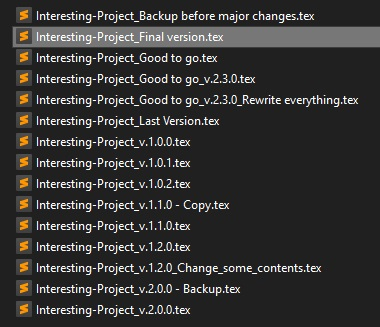
\includegraphics[height=6cm]{version_control} \nonumber
				\end{align}			
			\end{frame}

			\begin{frame}
				\frametitle{Version Control}
				\begin{itemize}
					\item A list of messy files, 
				\end{itemize}
			\end{frame}
		\subsection{What do we need for Version control?}
		\subsection{Git}

	\section{Git and GitHub}
		\subsection{Installation Git}
			\begin{frame}
				\frametitle{Installation}
				\begin{itemize}
					\item Windows: \url{https://git-scm.com/downloads}
					\item Linux: \texttt{sudo apt-get install git}
					\item Mac OS: 
						\begin{enumerate}
							\item Install \texttt{Xcode} from AppStore 
							\item Run \texttt{Xcode} 
							\item In \texttt{Xcode -> Preferences} find \texttt{Downloads} 
							\item Choose \texttt{Command Line Tools}, install it
						\end{enumerate}					
				\end{itemize}
			\end{frame}

			\begin{frame}
				\frametitle{Installation}
				After installation, open the terminal and input \texttt{git} to see if it is successfully installed. There should be something like this:
				\begin{align}
					\centering
					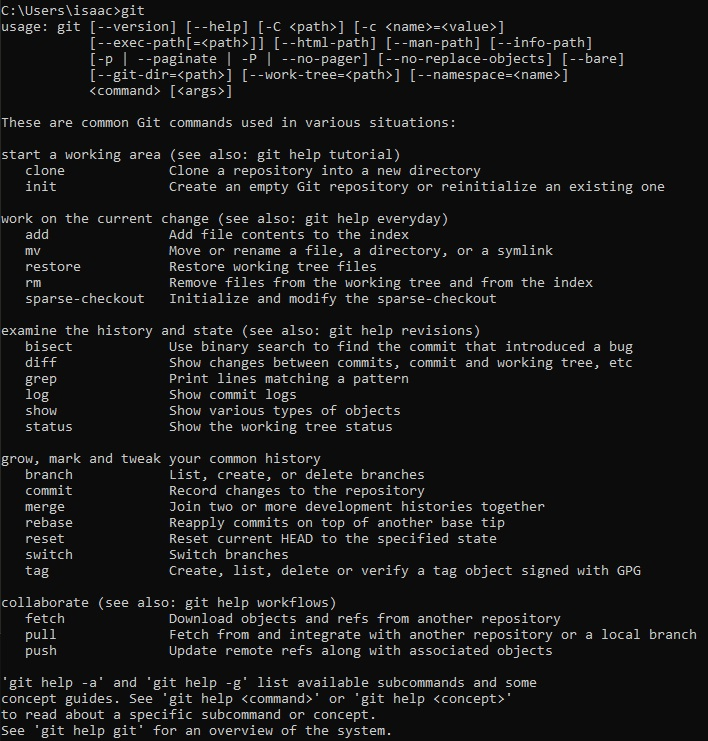
\includegraphics[height=5cm]{git_installed} \nonumber
				\end{align}
			\end{frame}
		\subsection{What is GitHub}
			\begin{frame}
				\frametitle{GitHub}
				\begin{itemize}
					\item A/the global company that provides hosting for software development version control using Git
					\item A website Microsoft just bought for \$7.5 billion dollar
					\item A website that you can guffy around when you are bored at coding and don't need to worry about getting caught by your manager (he/she might be doing the same thing)
				\end{itemize}
			\end{frame}

	\section{Using Git and GitHub}
		\subsection{Initialize/Clone}
			\begin{frame}
				\frametitle{Initialize/Clone}


			\end{frame}

		\subsection{Branch}
			\begin{frame}
				\frametitle{Branch}
			\end{frame}

		\subsection{Commit}
			\begin{frame}
				\frametitle{Commit}
			\end{frame}

		\subsection{Merge}
			\begin{frame}
				\frametitle{Merge}
			\end{frame}

			\begin{frame}
				\frametitle{Tip}
				\begin{itemize}
					\item Design by module
					\item Sync with master branch more often
					\item Commit with small changes (it depends)
				\end{itemize}
			\end{frame}

		\subsection{Revert/Reset}

		\subsection{.gitignore}

		\subsection{Pull request}

\end{document}